\section{Learning to Play a Game through Self-Play}
\subsection{Overview of the problem}
The final problem is to learn to play a game through self-play using parallel agents.  The focus is on the ultimate quality of the agent produced, with less emphasis on the speed of learning.  In this problem the agent is pre-programmed with knowledge about how the game works.  That is the agent can determine the next state of the game for any of the actions that are possible from the current state.  It also can determine which actions are legal actions from the current state.  The agent does not know the goal of the game and can not determine in advance what board positions are wins or losses, which must be learned through the reward signal.  The game uses the knight piece from chess on a 5 x 7 chessboard.  The game’s piece movement pattern, number of pieces per side, and board size are variable problem parameters but the results shown here are for knights on a 5 x 7 board and the game starts with the random placement of 5 pieces for each player.  Each player makes a move, as in chess, and a player wins if all opponent’s pieces are captured.  The game has a maximum number of turns and the result is a drawn game when that limit it is reached.

Learning through self-play was advanced by the famous work by Tesauro (Tesauro, 1994) who used TD($\lambda$) and self play to train a program to play backgammon at a master level.  This was dramatic accomplishment and has not yet been duplicated in other domains.  Tesauro points out in his work that it may be the random element that is present in backgammon that drives the learning agent into wide exploration of the state space, enabling high quality learning to take place during self-play.  The random element helps to avoid the problem of converging prematurely to a sub-optimal strategy that can happen with deterministic games.  In those games, the agent may only experience a small fraction of the state space and optimizes for this region only, since by playing itself, it never has to deal with other regions of the state space.

This game is discrete but has a large state/action space.  There are ${35 \choose 5} \times {30 \choose 5}$ possible starting positions with random placement of 5 Xs and 5 Os on a 5 by 7 board.  The total number of game states is even larger since pieces can be removed during the game.  The five knights can move in up to 8 directions each so there may be up to 40 possible actions.  Clearly, there are too many values to learn either $V(s)$ or $Q(s,a)$ for every point and generalization is required.  For this problem I chose to use a neural net to approximate the value function $V(s)$.  The value function can be used by the agent to pick optimal moves with one move look ahead.  The agent loops through possible moves, calculates the board position after each one and selects the move that results in the highest value board position.

\subsection{Neural Net Design}
The neural net must take a description of the board position and output the agent’s estimated value for that board position, $V(s)$.  I coded the board position as two series of binary values for each square on the board.  The first series had the value 1 when player X had a piece on the corresponding square and the second series indicated squares with an O piece.  A single layer of 4 hidden nodes with sigmoid activation is used and the single output node uses sigmoid activation as well.  The number of hidden nodes is a parameter that can vary.  The neural net design is shown Figure ???.

\end{flushleft}
\center
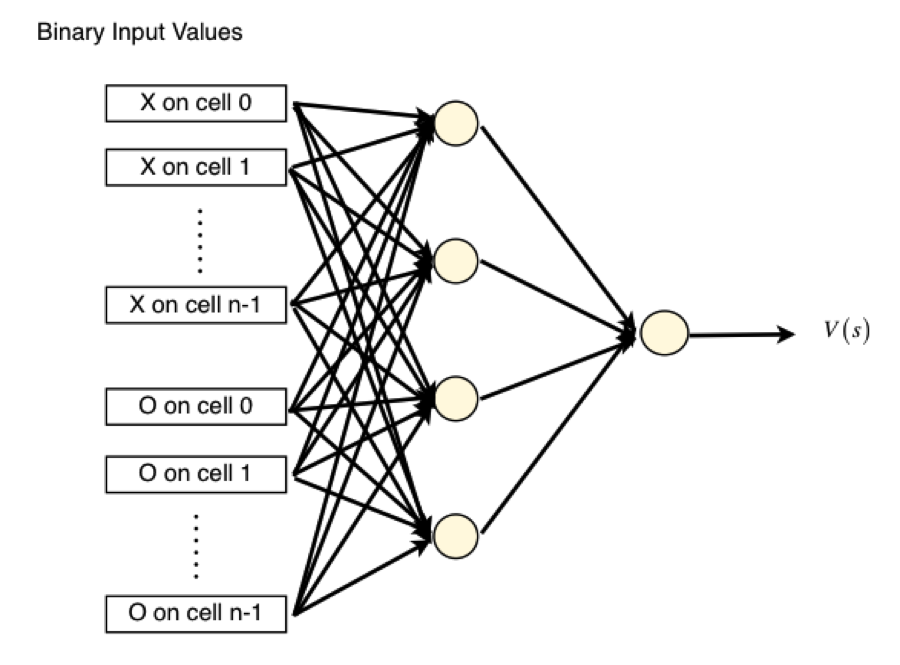
\includegraphics[scale=0.8]{fig11}
\begin{flushleft}

The learning algorithm for this problem is TD($\lambda$), building on the work done for the previous problems and adapting it to learn the $V(s)$ values.  The weight update rules combine the temporal difference equation for the value function with eligibility traces and back propagation updates for neural net weights.

The basic framework for learning is to have a group of agents learn by playing a set of games against each other.  The relative quality can be gauged by recording the agent’s winning percentage during the learning episodes.  This is shown for an 8-agent group in Figure 23.  The absolute measurement of agent quality requires some outside benchmark or test to be performed.  A benchmark opponent was used to gauge agent quality in Figure 24.  The quality measure is winning percentage calculated as $(wins + draws/2)/games$.

\end{flushleft}
\center
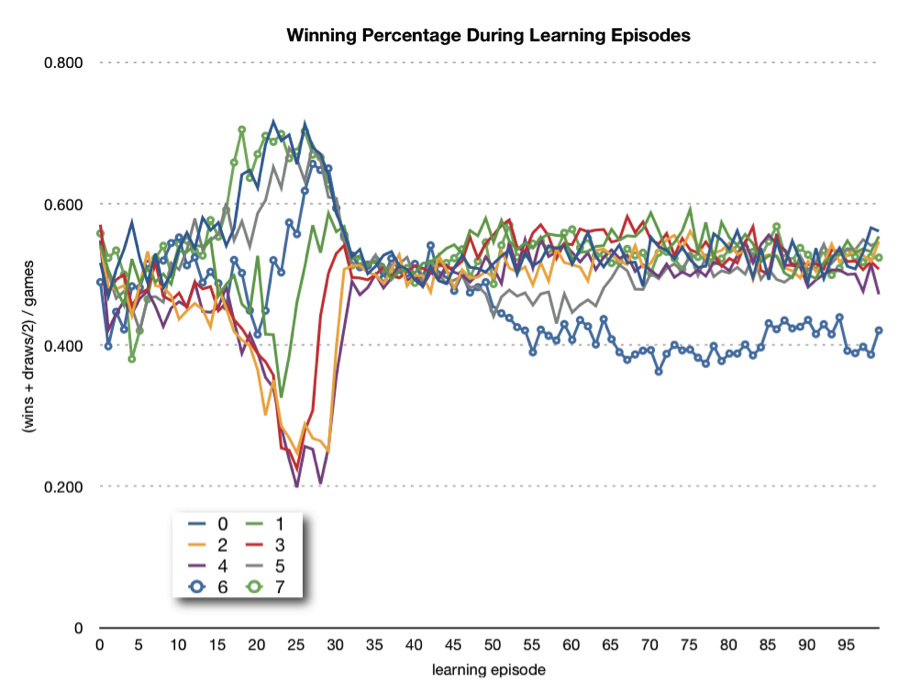
\includegraphics[scale=0.8]{fig12}
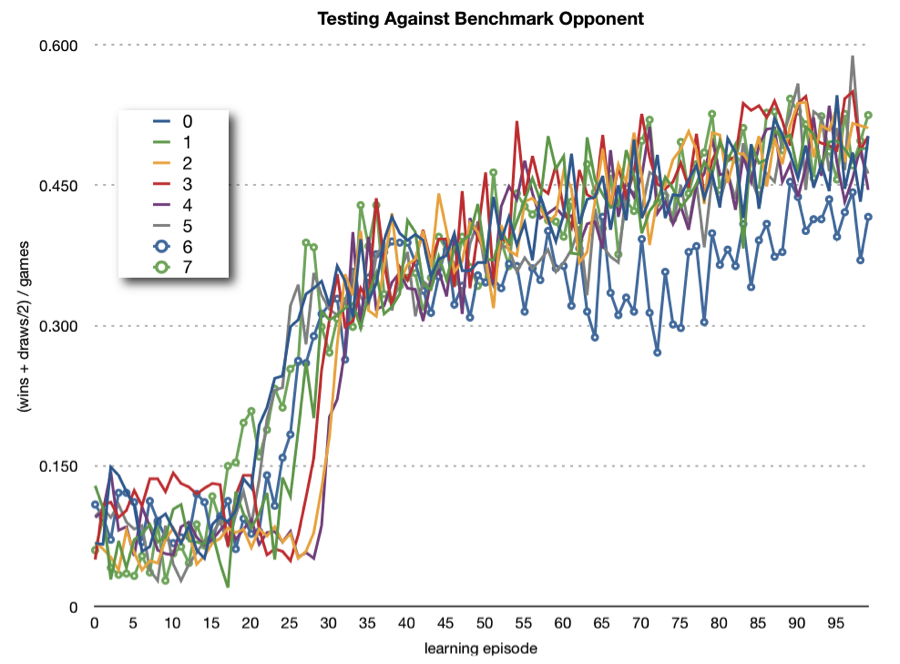
\includegraphics[scale=0.8]{fig13}
\begin{flushleft}


\subsection{GPU Implementation Issues}
The algorithm used on this problem is very compute intensive.  For each turn, the agent must look at all possible moves and estimate the value of the next board position by using the neural net estimate $V(s)$.  The GPU implementation uses multiple threads per agent to speed up the neural net calculations and to speed up the weight update calculations that are needed each turn.  Each agent has one thread per board square.  The entire group of threads within an agent will be active during some portions of the processing.  Other times, only a single thread or a smaller group of threads is needed for the calculations.  Thread activity for the choose move function is illustrated in Figure ???.  In that diagram, the green arrows represent active threads and dashed arrows are inactive threads.

\end{flushleft}
\center
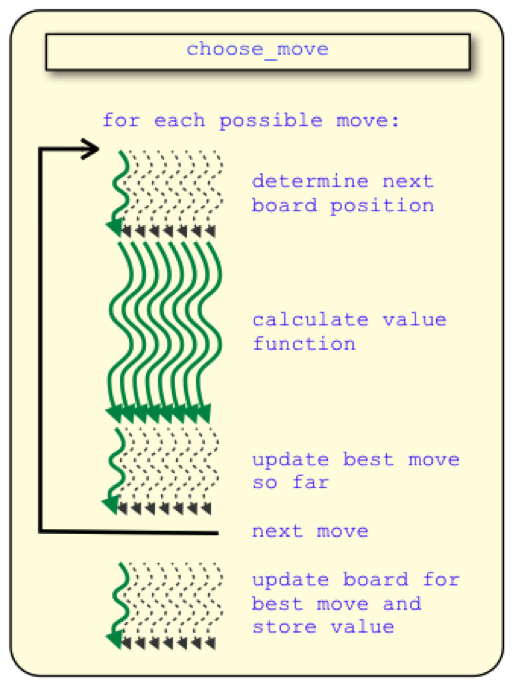
\includegraphics[scale=0.8]{fig14}
\begin{flushleft}


Agents can compete against an opponent in parallel too.  The next diagram, Figure ???, illustrates having $n$ agents compete against one opponent at the same time.

\end{flushleft}
\center
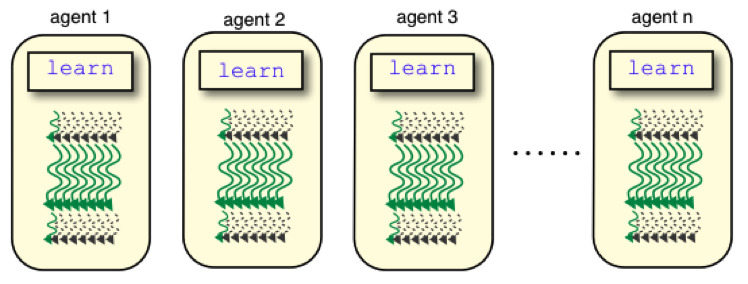
\includegraphics[scale=0.8]{fig15}
\begin{flushleft}

Having each agent compete against multiple opponents simultaneously increases parallelism further.  This approach requires creating multiple copies of the agent’s weights.  Each copy then competes against a different opponent and updates its own weights.  At the end of an episode of learning, the change in weights across all the copies of an agent is accumulated and the master copy is updated in one batch, illustrated in Figure ???.

\end{flushleft}
\center
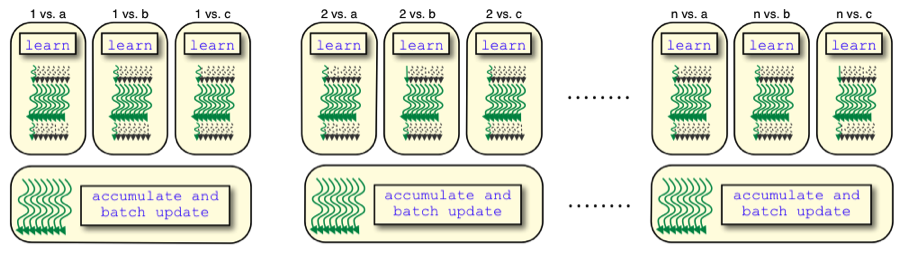
\includegraphics[scale=0.8]{fig16}
\begin{flushleft}


The processing on both the CPU and GPU is more complicated on this problem than on previous problems.  The GPU is much slower than the CPU for a single agent, but equals CPU speed with 4 agents and is faster for agent groups of 16 or more, as shown in Figure ???, which displays the learning time for one million turns.

\end{flushleft}
\center
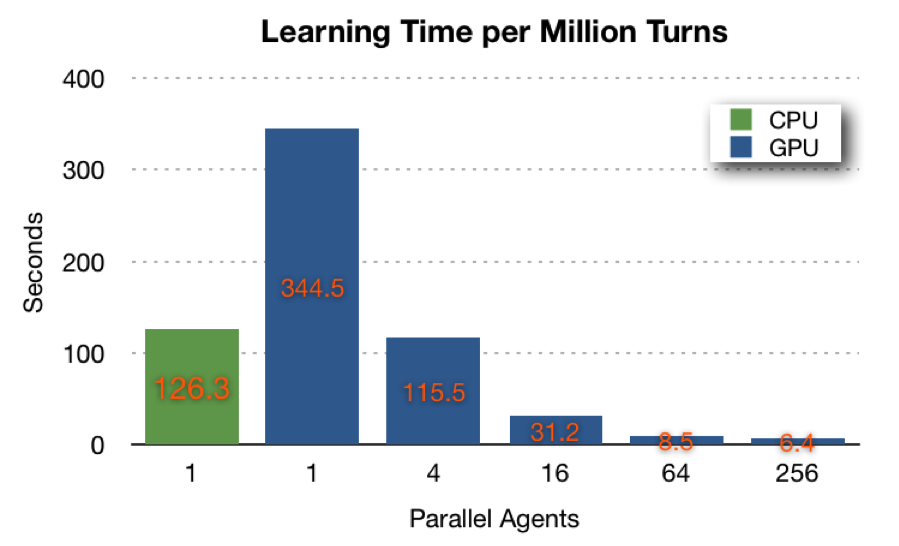
\includegraphics[scale=0.8]{fig17}
\begin{flushleft}



\subsection{Replication with Variation and Summary of Results}
There is no direct sharing between parallel agents in this problem.  Indirect sharing happens by agents competing against each other and learning.  If one agent’s quality improves, it becomes a better opponent for the other agents and the other agents should improve as a result as well.

This problem produces a wide variation of agent quality, similar to Mountain Car problem.  Selecting the best agent from a group of parallel agents, based on internal competition between agents or testing against a benchmark opponent, will improve the quality compared to the average result.  Variation in quality can be seen in Figure ???, which shows the best, worst, and average agent quality for a group of 64 parallel agents with quality measured against a benchmark opponent.

\end{flushleft}
\center
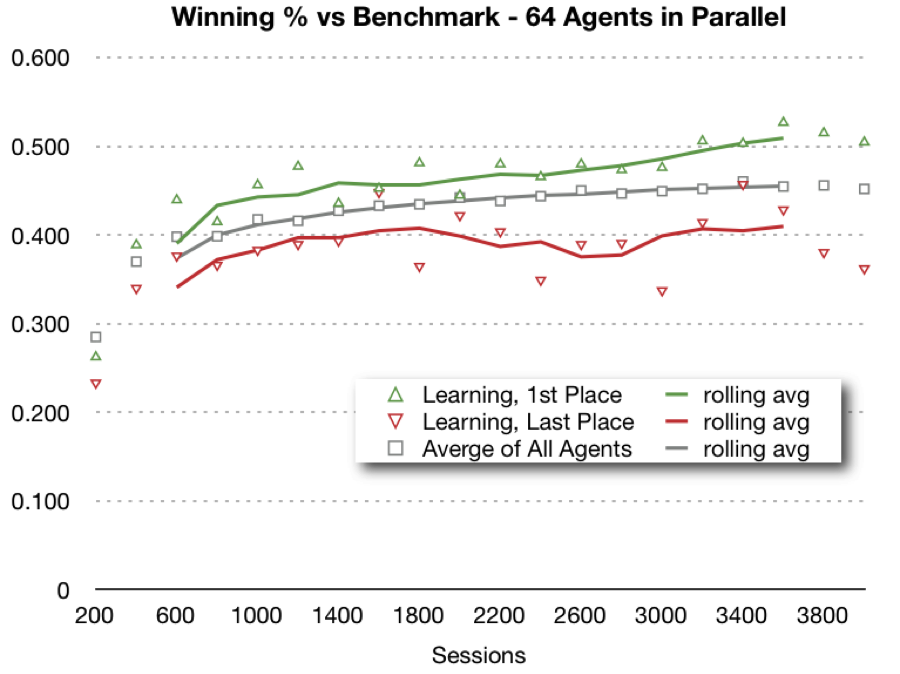
\includegraphics[scale=0.8]{fig18}
\begin{flushleft}


Another technique that works on this problem is the use of selective replication to improve the overall quality of the agent population.  After each learning episode a round-robin competition determines the relative quality of the agents.  The best agents are copied and the worst agents dropped.  In addition, this has a secondary effect of improving the opponents for all agents in the future.  Figure ??? shows the high-level sequence diagram for CPU and GPU coordination.

\end{flushleft}
\center
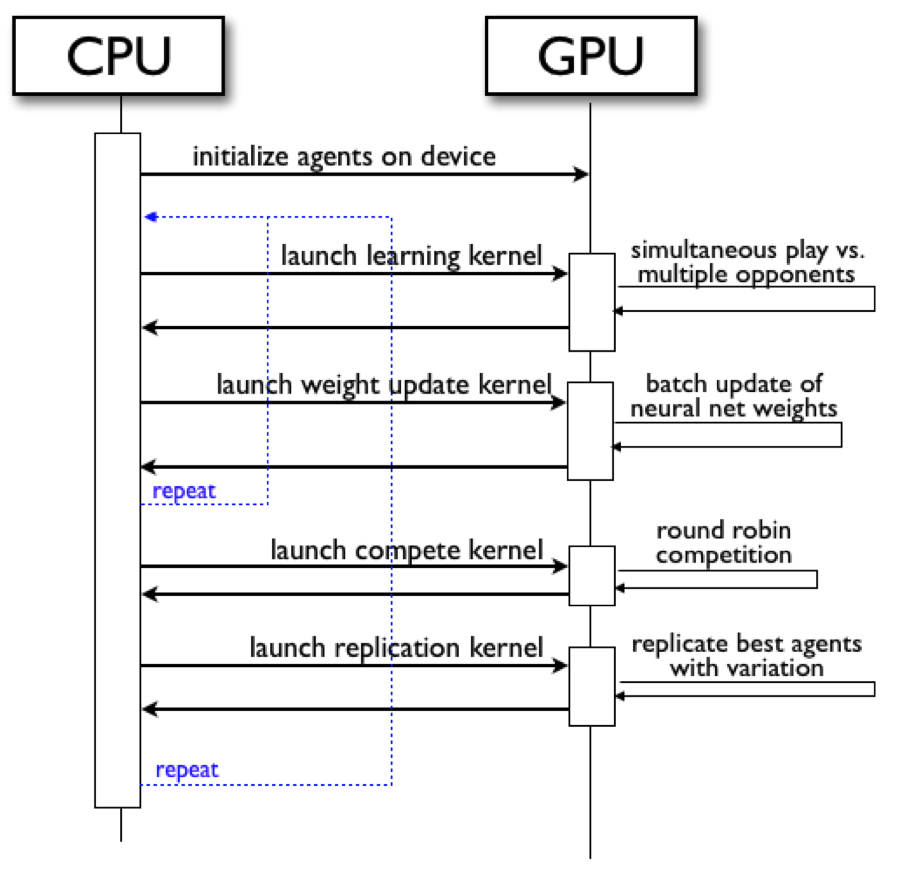
\includegraphics[scale=0.8]{fig19}
\begin{flushleft}

The replicated copies of the best agents can include some differentiation.  They can have variation in the learning parameters or slight random bias applied to the neural net weights.  Variation helped the population of agents to continue to improve over a long training session.  The last graph, Figure ???, shows the typical results when using selective replication with variation with a group of 64 agents.  

\end{flushleft}
\center
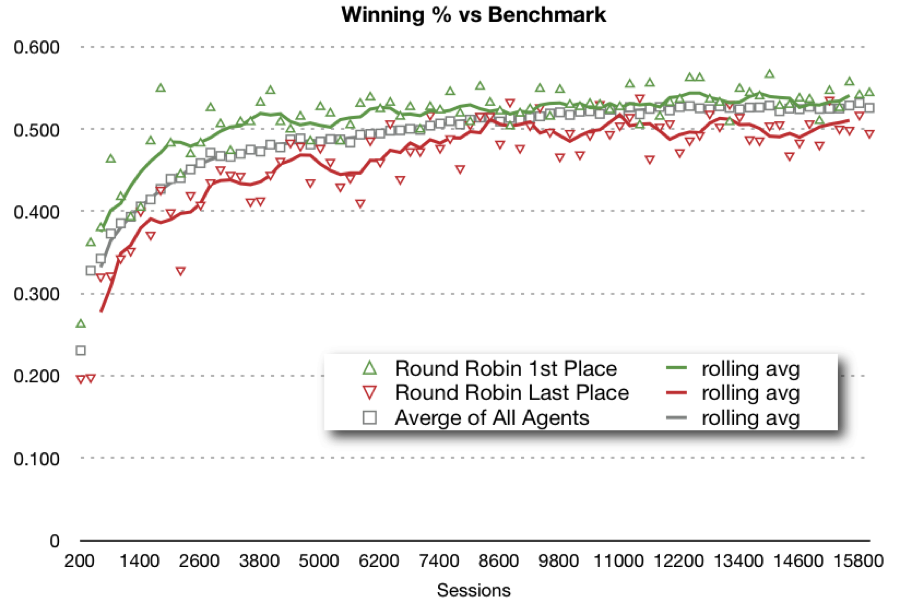
\includegraphics[scale=0.8]{fig20}
\begin{flushleft}


The parallel approach to this problem provides a variety of opponents for agents to learn from.  This can help overcome the problems with self-play using a single agent.  In addition, the evolutionary techniques of selective replication with variation allow the population of agents to continue to improve over time.

%\section{Prior Work}

Parallelism techniques have been applied to reinforcement learning in the past.  These applications typically ran on CPUs, but more recently, running on GPUs.  There are also a number of different ways parallelism can be applied.

There are many works that combine multiple agents and reinforcement learning to address a multiagent learning problem.  A Comprehensive Survey of Multiagent Reinforcement Learning ~\cite{Busoniu:2008p4935} describes some of the work in this area.  In contract, this thesis addresses what are traditionally single agent learning problems, and parallelism is used to find the highest quality single agent as fast as possible.  The output of the techniques in this thesis is a single agent even though multiple agents may be used in parallel to find it.

V. Palmer ~\cite{Palmer:2007p4912} used GPU programming to speed up matrix calculations in the Least Squares Policy Iteration algorithm ~\cite{Lagoudakis:2003p4913} applied to a multi-agent cooperative Pole Balancing problem.  The GPU was used to speed up calculations on a fixed set of training data for from 1 to 4 agents where each agent had 20 basis functions.  Here, the parallelism on the GPU was used to get a computational speed up of the policy evaluation and policy improvement steps of the Least Squares Policy Iteration algorithm for each agent.  The implementation and interaction of multiple agents was done on the CPU.  The batch processing using the GPU was compared to a Matlab implementation and found to improve calculation speed for training sets of at least 400 points.  The GPU calculation time grew much slower than the CPU calculation time as the training set increased and also as the number of agents increased.

In this thesis we use the GPU to implement parallelism across multiple agents.  In Palmer’s study, the GPU was used within each agent to speed up that agent’s calculations, but did not attempt to deal with multiple cooperating agents with varying experience and the issues of data communication on the GPU.  Furthermore, the degree of parallelism applied in thesis is much greater, with agent group sizes in hundreds or thousands compared to a maximum of 4 agents in Palmer.

Grounds and Kudenko used a parallel approach with multiple CPUs for three reinforcement learning problems ~\cite{Grounds:2008p3736}.  They parallelized across agents and studied the communication issues between multiple agents.  In their approach, each agent communicated its information to all other agents in a staggered fashion over time.  The agents took turns broadcasting their information to the other agents.  The information communicated was limited to the most important parameters learned by that agent.  The importance of a parameter was determined by how much it changed since the previous communication.  Reducing the quantity of data communicated was necessary due to the relatively slow communication speed between CPUs running on separate machines.  They tested from 1 to 16 agents on Pole Balancing, Mountain Car, and a Grid World problem, and demonstrated increasing quality of learning for a given training time as the number of agents increased.

This thesis differs by running the parallel agents on a single GPU instead of multiple CPUs.  The GPU makes it possible to use thousands of agents while Grounds and Kudenko used a maximum of 16 agents.  Kudenko had to severely limit the quantity of information shared between agents because of the high cost of communication between processes running on different CPUs, which is less of a problem for this thesis.  On the GPU the cost of communication is simply the cost of synchronizing all agents at a sharing point and then calculating and storing values in global memory on the GPU.  Communicating between threads on a single GPU can be less time consuming than communicating between processes on different CPUs.

Kretchmar ~\cite{Kretchmar:2002p3812} applied a parallel approach to the N-armed Bandit problem, which we introduce in Chapter 4.  Kretchmar used from 1 to 10 agents in parallel and the quality of learning was measured as a function of time steps per agent. After each time step, all agents shared information.  Individual agents kept track of their own experience data and that of all other agents separately.  This approach allowed the agents to share just the data from their own experience while still having access to the combined information.  The results showed improved learning quality as the number of agents increased as a function of the number of steps in the learning process.  Measurements were made as a function of action steps per agent, so total actions taken increased as the number of agents was increased.  Results were not timed so the cost of communication between agents was not reflected in the quality measurements.

Kretchmar did not consider the time cost involved with parallel agents and information sharing, and by sharing after every time step the agents had complete information.  In this thesis, time is an important component when measuring of the quality of learning. In this work agents spent most of the time operating independently, agents only share information periodically, and the agents do not have complete information. 

Evolutionary techniques are a natural subject when multiple agents are used.  Evolutionary methods and reinforcement learning are compared in ~\cite{Whiteson:2010p4931}.  In that work the methods are each applied to two learning problems and the problem characteristics which favor reinforcement learning or evolutionary learning are discussed.  Evolutionary methods and reinforcement learning are considered distinct approaches to solving a learning problem.  In this thesis, we combine some evolutionary techniques with the reinforcement learning process implemented by multiple agents, with beneficial results.

The main differences between this thesis and prior work is the use of the GPU to apply massive parallelism to reinforcement learning problems allowing the use of hundreds or thousands of agents. Large numbers of parallel agents are shown to able to improve the reinforcement learning process through a number of techniques.  Empirical measurements are made to demonstrate the improved learning due to information sharing, differentiation, and evolution of hundreds or thousands of agents.




